\documentclass[12pt]{article}

\usepackage{times,mathptmx}
\usepackage[pdftex]{graphicx}
\usepackage{pdflscape}

\usepackage{subcaption}
\usepackage{graphicx}
\usepackage{float}
\usepackage[section]{placeins}
\usepackage{fancyhdr}
\usepackage{enumitem}
 %\usepackage[none]{hyphenat}

\usepackage{tocloft}
\usepackage[nottoc,notlof,notlot]{tocbibind} % Put the bibliography and index in the ToC

\pagestyle{fancy}
\rhead{}
\lhead{}
\chead{}
\cfoot{Page \thepage}
%\renewcommand{\headrulewidth}{0.4pt}
\renewcommand{\footrulewidth}{0.4pt}

\usepackage{color}
\usepackage{amsmath}
\usepackage{multirow}
\definecolor{linknavy}{rgb}{0,0,0.50196}
\definecolor{linkred}{rgb}{1,0,0}
\definecolor{linkblue}{rgb}{0,0,1}

\usepackage{xr-hyper}
\usepackage[pdftex,
        colorlinks=true,
        urlcolor=linkblue,     % \href{...}{...} external (URL)
        citecolor=linkred,     % citation number colors
        linkcolor=linknavy,    % \ref{...} and \pageref{...}
        pdfproducer={pdflatex},
        pagebackref,
        pdfpagemode=UseNone,
        bookmarksopen=true,
        plainpages=false,
        verbose]{hyperref}

\setlength{\textwidth}{6.7in}
\setlength{\textheight}{9.0in}
\setlength{\topmargin}{0.in}
\setlength{\headheight}{0.0in}
\setlength{\headsep}{0.1in}
\setlength{\parindent}{0.25in}
\setlength{\oddsidemargin}{-0.1in}
\setlength{\evensidemargin}{0.0in}




\begin{document}
\begin{center}

\section*{Call for Participation in the MaCFP-4 Workshop}
%\begin{figure}[h]
%  \centering
%  \includegraphics[width=3in]{../../Figures/MaCFP_Logo.pdf}
%  \label{Cover_Image}
%\end{figure}
{\large || June, 2026   |   La Rochelle, France ||}
\end{center}

\subsection*{Target Cases} 
\label{Target Cases}
\small
The fourth Measurement and Computation of Fire Phenomena Workshop (MaCFP-4) is scheduled to take place prior to the 15th IAFSS Symposium, which will be held June 8-12, 2026 in La~Rochelle, France. This call for participation provides a summary of MaCFP-4 target cases and a preliminary schedule of the events leading up to the Workshop (including virtual meetings).\\

\textbf{Radiation:}
\begin{itemize} [noitemsep]
    \item \underline{Prediction of radiation fields of benchmark combustion systems.} Predictions made by the radiation solvers of fire CFD codes will be compared against experimental heat fluxes and synthetic data (net source term, emission, absorption) obtained from Particle Monte Carlo - Line-by-line (PMC-LBL) calculations of a 30~cm methanol pool flame (HRR~=~19.2~kW) and a 15~cm ethylene diffusion flame (HRR~=~15~kW). 
\item \underline{Characterization of absorption and emissivity of a charring material.} The Radiation Subgroup will  help to coordinate the Condensed Phase Subgroup's pyrolysis model calibration exercise.
\end{itemize}

\textbf{Condensed Phase:}
\begin{itemize} [noitemsep]
    \item \underline{Pyrolysis model calibration of a charring material: pine wood.}
    No single approach is suggested for model parameterization. In fact, a key objective of this material property determination exercise is to catalog current approaches used to parameterize complex pyrolysis models. \emph{Experimentalists} are asked to perform tests and share their measurement data to be made publicly available on the \href{https://github.com/MaCFP/matl-db/tree/master/Wood}{MaCFP GitHub Repository}. \emph{Modelers} are asked to calibrate material property sets using this data and perform simulations of material response to heating (0D thermal decomposition and 1D gasification). Limited quantities of the test material will be made available directly to participants who can commit to conducting certain experiments. MaCFP-4 pyrolysis modeling targets will include $only$ anaerobic conditions; however, participants are encouraged to develop experimental datasets and corresponding models that will describe oxidation (as will be studied in detail at MaCFP-5).\\
\end{itemize}

\textbf{Gas Phase:}
\begin{itemize} [noitemsep]
\small
    \item \underline{\href{https://github.com/MaCFP/macfp-db/tree/master/Extinction/FM_Burner}{FM Burner}.} Study of soot formation/oxidation and thermal radiation transport in turbulent buoyant diffusion flames using existing data; this dataset features different oxidizer conditions and different fuels. The FM Burner configuration was developed and studied at FM.
    \item \underline{Upward flame spread.} Systematic, constrained modeling study of flame structure/heat flux and fire growth over MaCFP-PMMA. This study considers existing data from two configurations based on:\\
    (1) the FM~4910 fire test, as studied at NIST (called NIST-data{\_}FM4910-config); and\\
    (2) the EN 13823 Single Burning Item (SBI) fire test, as studied at UMD (called UMD-data{\_}SBI-config).
    \item \underline{Compartment/façade fires.} Study of flame structure and heat transfer using existing data [Sun et al.~(2024) Fire and Materials, 48.4:411-425]. The database features 1-MW-scale compartment fires and external flames and spill plumes thermally loading a vertical inert façade. This configuration is based on the JIS~A~1310 fire test, as studied at the Building Research Institute (BRI) of Japan and the University of Tokyo (UoT) (called BRI-UoT-data{\_}JISA1310-config). 
%    \item \underline{`Blind' study of flame spread and fire growth over wood.} {\color{red} A configuration based on the FM 4910 fire test and studied at NIST (called NIST{\_}data{\_}FM4910{\_}config{\_}wood{\_}mat).} At MaCFP-4, pine wood will be characterized in micro-scale and bench-scale experiments focusing on pyrolysis (without char oxidation). At MaCFP-5, this material will be characterized in micro-scale and bench-scale experiments including char oxidation, as well as in flame spread and fire growth experiments using a parallel panel configuration; different separation distances between the panels will be considered. 
\end{itemize}

\clearpage
\normalsize
\subsection*{Workshop Timeline (Tentative)} 
\label{Timeline}
\small
\begin{table} [h!]
\begin{tabular}{p{0.16\linewidth} | p{0.84\linewidth}}
\hline
\textbf{Date}          & \textbf{Objective} \\
\hline
% Feb. 26, 2025 		& Release \href{https://github.com/user-attachments/files/18370197/MaCFP-2_Proceedings_GasPhase.pdf}{MaCFP-2 Proceedings}\\
% \\
March 21, 2025  	& Share `Call for Participation in MaCFP-4' Document\\
    & Share `Guidelines for Participation in MaCFP-4' Document \\
    %& Share MaCFP-3 Proceedings (Final Draft) for public comment\\
    & Call for participation (modelers) in radiation cases\\
    & Call for participation (experimentalists) in pyrolysis model calibration exercise\\
\\
%\textcolor{red}{Feb. 4, 2025}         	& \textcolor{red}{Virtual meeting (Radiation/Gas Subgroup; all participants welcome)}\\
%\textcolor{red}{11:30 AM (EST)}   	& \textcolor{red}{Present details of four target cases; highlight cases \# and \#\# for October Virtual meeting}\\
%\\
March 28, 2025         & Virtual meeting (all participants welcome)\\
9:00 AM (EST)   	& Present details of pyrolysis model calibration exercise (material information, how to request samples; test data of interest, formatting and submission requirements)\\
& Present details of radiation modeling exercise (prediction of radiation fields of benchmark combustion systems)\\
\\
Spring 2025  	& Coordinate distribution of material samples for pyrolysis model calibration exercise\\
\\
%\hline
%Sept. 5, 2025       	& Deadline to submit modeling results (Gas Phase)\\
Nov. 2025        	& Deadline to submit measurement data (Pyrolysis Experiments)\\
				& Call for volunteers [repo management, data analysis, scripting, etc.]\\
\\
\hline 
% \multicolumn{2}{c}{ Virtual Meeting (`MaCFP-3.5')}\\
% \hline
%\textcolor{red}{Oct. 21, 2025}		& \textcolor{red}{Virtual meeting (Radiation/Gas Subgroups; all participants welcome)}\\
%& \textcolor{red}{Co-chairs of rad-/gas-phase, can we present Case 3?}\\
\textbf{Jan. 14, 2025}	& \textbf{Virtual Meeting (`MaCFP-3.5')}\\
& Coordinated by Condensed Phase Subgroup, all participants welcome\\
& Summary of experimental data submitted to pyrolysis model calibration exercise\\
                       		& Call for participation (modelers) in pyrolysis model calibration exercise\\
                            \\
% \hline
Feb. 13, 2026       	& Share final `Guidelines for Participation in MaCFP-4' document\\
				& Deadline to submit revisions to experimental datasets (pyrolysis model calibration)\\
\\
May 9, 2026       	& Deadline to submit pyrolysis model calibration results (Condensed Phase Subgroup)\\
                & Deadline to submit radiation modeling results (Radiative Heat Transfer Subgroup)\\
            & Deadline to submit modeling results (Gas Phase Subgroup, all cases)\\ 
				& Poster abstract deadline (MaCFP-4 experimental data and modeling submissions) \\
%Spring 2026	        	& Virtual Meeting  (Condensed Phase Subgroup; all participants welcome):\\
%                    		& Comparisons of derived pyrolysis parameters and parameter sets \\
% 				& Comparisons of pyrolysis model predictions\\
\\

\hline
\textbf{June, 2026}       	& \textbf{MaCFP-4 Workshop: La Rochelle, France} \\
\hline
\end{tabular}
\end{table}
\normalsize

\begin{figure}[h!]
  \centering
  \includegraphics[width=3.1in]{../MaCFP_Logo.pdf}
  \label{Cover_Image}
\end{figure}


\end{document}
